\section{Introduction}
\label{sec:introduction}

% state the learning objective
The objective of this laboratory assignment was to study a circuit made up of a two voltage sources (one dependent), two current sources (one dependent) and seven resistors. It can be seen in the Figure ~\ref{circuit} below.

In Section~\ref{sec:analysis}, a theoretical analysis of the circuit is presented. It is followed by a simulation of the circuit, in Section~\ref{sec:simulation}, the results of which are compared to the theoretical results in the final section, Section~\ref{sec:conclusion}. Here, some  considerations are also made about this study, the results obtained and whether the goals were achieved.

In order to conduct the theoretical study, the tool {\bf Octave} was employed. The simulation was run in {\bf Ngspice}. In order to numerically assess the results, a {\bf Python} {\it script} was also used.

%In Section~\ref{sec:analysis}, a theoretical analysis of the circuit is presented. In Section~\ref{sec:simulation}, the circuit is analysed by simulation, and the results are compared to the theoretical results obtained in Section~\ref{sec:analysis}. The conclusions of this study are outlined in Section~\ref{sec:conclusion}.

\begin{figure}[H]
  \centering
  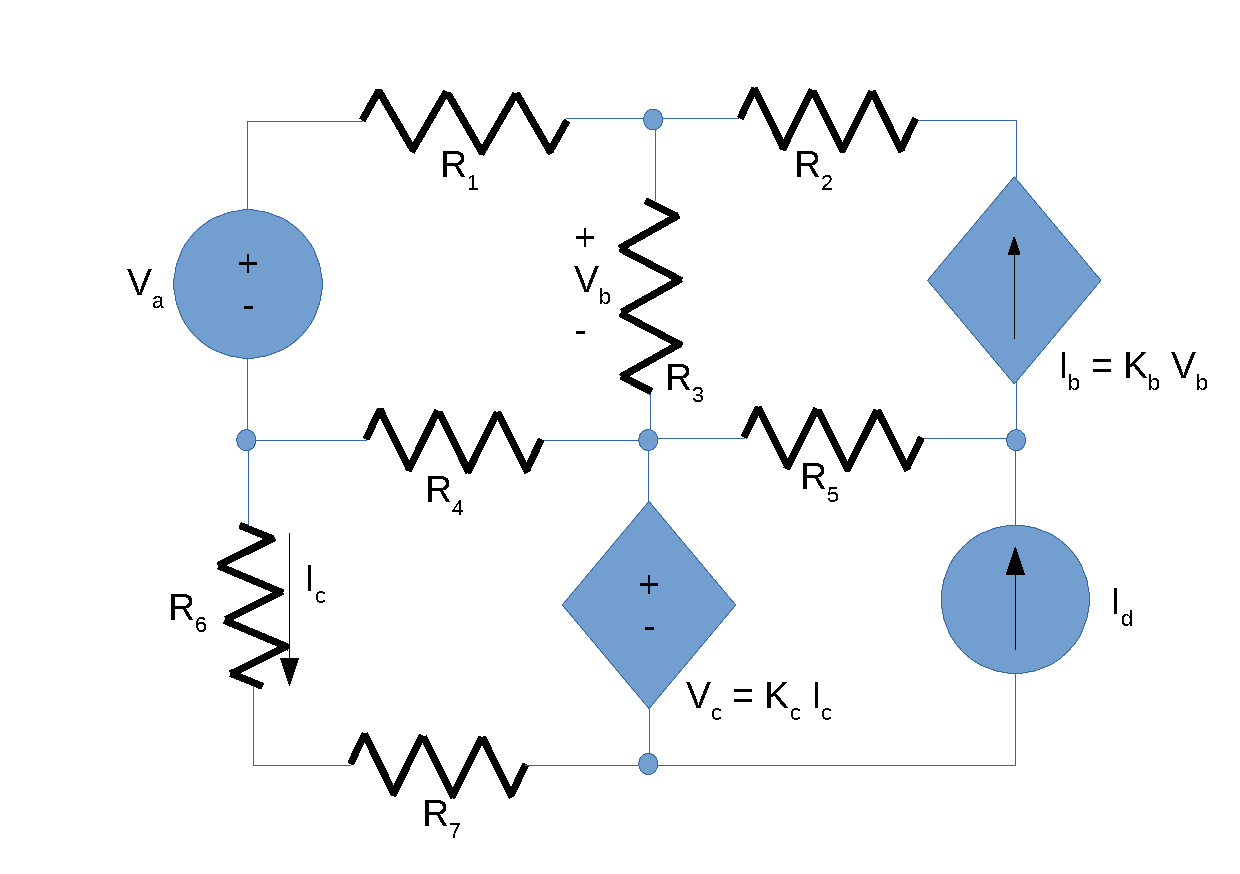
\includegraphics[width=0.6\linewidth]{simple.pdf}
  \caption{Circuit considered}
  \label{circuit}
\end{figure}

